\begin{lemma} \leavevmode \\
    \label{lemma6.5}
    Suppose $f:[a,b] \to \R$ is bounded, $\alpha: [a,b] \to \R$ is increasing, $P = \set{x_0,...,x_n} \in \Pi[a,b]$, and $R \in \R$.
    \begin{enumerate}
        \item If for all tags $(s_k)_{a \leq k \leq n}$ of $P$ we have $\sum_{k=1}^{n}f(s_k)\Delta\alpha_k \leq R,$ then $U(f, \alpha, P) \leq R$.
        \item If for all tags $(s_k)_{a \leq k \leq n}$ of $P$ we have $R\leq \sum_{k=1}^{n}f(s_k)\Delta\alpha_k$, then $L(f, \alpha, P) \geq R$.
    \end{enumerate}
\end{lemma}

\begin{proof}
    \begin{enumerate}
        \item If $\alpha$ is constant, then $\sum_{k=1}^{n}f(s_k)\Delta \alpha_k = 0$ and $U(f, \alpha, P) = \sum_{k=1}^{n}M_k \Delta \alpha_k = 0,$ so the claim obviously holds. Suppose $\alpha(b) \neq \alpha(a)$. It's enough to show
        $$\forall \epsilon > 0 ~~U(f, \alpha, P) \leq R + \epsilon.$$
        Let $\epsilon > 0$ be given. For each $k \in \set{1, ..., n}$ we have
        $$M_k = \sup\set{f(x) : x \in [x_{k-1}, x_k]} \implies \exists s_k \in [x_{k-1}, x_k] \st M_k -\frac{\epsilon}{\alpha(b) - \alpha(a)} < f(s_k).$$
        We have 
        \begin{align*}
            U(f,\alpha, P) &= \sum_{k = 1}^{n}M_k \Delta \alpha_k < \sum_{k=1}^{n}\left[f(s_k) + \frac{\epsilon}{\alpha(b) - \alpha(a)}\right]\Delta \alpha_k \\
            &=\sum_{k=1}^{n}f(s_k)\Delta \alpha_k + \frac{\epsilon}{\alpha(b) - \alpha(a)}\sum_{k=1}^{n}\Delta \alpha_k \\
            &\leq R + \epsilon
        \end{align*}
        as desired.

        \item Completely analogous to (i).
    \end{enumerate}
    \qed
\end{proof}

\begin{theorem} \leavevmode \\
    \label{Thm6.17}
    Suppose $f:[a,b] \to \R$ is bounded, $\alpha[a,b]\to \R$ is increasing, and $\alpha' \in R[a,b].$ Then
    $$f \in R_\alpha[a,b] \iff f\alpha'\in R[a,b]$$
    and in this case,
    $$\int_a^bf d\alpha = \int_a^b f(x)\alpha'(x) dx.$$
\end{theorem}

\begin{proof}
    It is enough to show that
    \begin{align*}
        U(f, \alpha) = U(f\alpha') \tag{$*$} \\
        L(f, \alpha) = L(f\alpha')
    \end{align*}
    Indeed, if we prove ($*$), then we can write
    \begin{align*}
        f\in R_\alpha[a,b] &\iff U(f, \alpha) = L(f, \alpha) \\
        &\iff U(f\alpha') = L(f\alpha') \\
        &\iff f\alpha' \in R[a,b].
    \end{align*}
    Moreover,
    $$\int_a^bfd\alpha = U(f, \alpha) \overset{(*)}{=} U(f\alpha') = \int_a^b f(x) \alpha'(x)dx.$$
    In what follows, we will prove $U(f,\alpha) = U(f\alpha')$. The proof for $L(f,\alpha) = L(f\alpha')$ is completely analogous. let $P = \set{x_0, ..., x_n}$ be any partition of $[a,b]$. Let $(s_k)$ be any tag of $P$. We have
    \begin{align*}
        \left|\sum_{k=1}^{n}f(s_k)\Delta \alpha_k - \sum_{k=1}^{n}f(s_k)\alpha'(s_k) \Delta x_k\right| &= \left|\sum_{k=1}^{n}f(s_k)\alpha'(t_k)\Delta x_k - \sum_{k=1}^{n}f(s_k)\alpha'(s_k) \Delta x_k\right| \tag{MVT on $\Delta\alpha_k$} \\
        &= \left|\sum_{k=1}^{n}f(s_k) \left(\alpha'(t_k) - \alpha'(s_k)\right)\Delta x_k\right| \\ 
        &\leq \sum_{k=1}^{n}|f(s_k)| \cdot \left|\alpha'(t_k) - \alpha'(s_k)\right| \Delta x_k \\
        &\leq \hat{M} \sum_{k=1}^{n}\left|\alpha'(t_k) - \alpha'(s_k)\right|\Delta x_k \tag{$\hat{M}=\sup_{a \leq x \leq b}|f(x)|$} \\
        &\leq \hat{M} \sum_{k=1}^{n}\left[\sup_{I_k}\alpha' - \inf_{I_k}\alpha'\right]\Delta x_k \tag{Lemma \ref{lemma6.1}} \\
        &= \hat{M} \left[U(\alpha', P) - L(\alpha', P)\right]
    \end{align*}
    So,
    $$\left|\sum_{k=1}^{n}f(s_k)\Delta \alpha_k - \sum_{k=1}^{n}f(s_k)\alpha'(s_k)\Delta x_k\right| \leq \hat{M}\left[U(\alpha', P)- L(\alpha', P)\right].$$
    Therefore,
    \begin{align*}
        (1)~~ \sum_{k=1}^{n}f(s_k) \Delta \alpha_k &\leq \sum_{k=1}^{n}f(s_k)\alpha'(s_k)\Delta x_k + \hat{M} \left[U(\alpha', P) - L(\alpha', P)\right] \\ 
        &\leq U(f\alpha', P) + \hat{M}\left[U(\alpha', P) - L(\alpha', P)\right].
    \end{align*}
    So, by Lemma \ref{lemma6.5},
    $$U(f, \alpha, P) \leq U(f\alpha', P) + \hat{M}\left[U(\alpha', P) - L(\alpha', P)\right].$$
    \begin{align*}
        (2)~~ \sum_{k=1}^{n}f(s_k)\alpha'(s_k) \Delta x_k &\leq \sum_{k=1}^{n}f(s_k) \Delta \alpha_k + \hat{M}\left[U(\alpha', P)-L(\alpha', P)\right]
    \end{align*}
    So, by Lemma \ref{lemma6.5},
    $$U(f\alpha', P) \leq U(f, \alpha, P) + \hat{M}\left[U(\alpha', P)-L(\alpha',P)\right].$$
    It follows from (1) and (2) that 
    $$(3)~~ \left|U(f, \alpha, P) - U(f\alpha', P)\right| \leq \hat{M}\left[U(\alpha', P) - L(\alpha', P)\right].$$
    Note that
    \begin{align*}
        U(f, \alpha) = \inf\set{U(f, \alpha, P) : P \in \Pi} &\implies \exists (P^{(1)}_n)\subseteq \Pi \st \lim_{n \to \infty}U(f, \alpha, P^{(1)}_n) = U(f, \alpha) \\
        U(f\alpha') = \inf\set{U(f\alpha',P) : P \in \Pi} &\implies \exists (P^{(2)}_n)\subseteq \Pi \st \lim_{n\to \infty} U(f\alpha', P^{(2)}_n) = U(f\alpha') \\
        \alpha' \in R[a,b] &\implies \exists (P^{(3)}_n) \subseteq \Pi \st \lim_{n\to \infty}\left[U(\alpha', P^{(3)}_n)-L(\alpha', P^{(3)}_n)\right] = 0.
    \end{align*}
    For each $n \in \N$, let $P_n = P^{(1)}_n \cup P^{(2)}_n \cup P^{(3)}_n.$ By the Squeeze Theorem,
    \begin{align*}
        \forall n \geq 1 ~~U(f, \alpha) \leq U(f, \alpha, P_n) \leq U(f, \alpha, P^{(1)}_n) &\implies \lim_{n\to \infty} U(f, \alpha, P_n) = U(f, \alpha) \\ 
        \forall n \geq 1 ~~U(f\alpha') \leq U(f\alpha', P_n) \leq U(f\alpha', P^{(2)}_n) &\implies \lim_{n \to \infty} U(f\alpha', P_n) = U(f\alpha').
    \end{align*}
    Since $P_n$ is a refinement of $P^{(3)}_n$,
    $$0 \leq \left[U(\alpha', P_n) - L(\alpha', P_n)\right] \leq U(\alpha', P^{(3)}_n) - L(\alpha', P^{(3)}_n) \implies \lim_{n \to \infty} \left[U(\alpha', P_n)-L(\alpha', P_n)\right] = 0.$$
    It follows from (3) that 
    $$\forall n \geq 1 ~~0 \leq \left|U(f, \alpha, P_n) - U(f\alpha', P_n)\right| \leq \hat{M}\left[U(\alpha', P_n) - L(\alpha', P_n)\right].$$
    So, by the Squeeze Theorem,
    \begin{align*}
        &\lim_{n\to \infty}\left|U(f, \alpha, P_n) - U(f\alpha', P_n)\right| = 0 \\
        \implies &\left|\lim_{n\to \infty}\left(U(f, \alpha, P_n) - U(f\alpha', P_n)\right)\right| = 0 \\
        \implies &\left|U(f, \alpha) - U(f\alpha')\right| = 0 \\
        \implies &U(f, \alpha) - U(f\alpha') = 0 \\
        \implies &U(f,\alpha) = U(f\alpha') 
    \end{align*}
    \qed
\end{proof}

\begin{theorem}[Change of Variables for Integrals] \leavevmode \\
    \label{Thm6.19}
    Let $f \in R_\alpha[a,b],$ and let $\phi: [A,B]\to [a,b]$ be onto and strictly increasing. If we let $g = f \circ \phi$ and $\beta = \alpha \circ \phi$, then
    $$g \in R_\beta[A,B] \text{ and } \int_a^bfd \alpha = \int_A^Bg d \beta.$$
\end{theorem}

\begin{remark}
    Consider the special case where $\alpha(x) = x$ and $\phi' \in \R.$ In this case, $\beta = \alpha \circ \phi = \phi.$ So, the conclusion of the theorem can be written as
    $$\int_a^bf(x)dx = \int_A^B(f\circ \phi)d\phi = \int_A^Bf(\phi(y))\phi'(y)dy.$$
\end{remark}

\colorlet{proofcolor}{theorembordercolor}
\begin{proof}
    First, note that
    $$\begin{rcases*}
        \alpha:[a,b] \to \R \text{ is increasing } \\
        \phi: [A,B] \to \R \text{ is increasing }
    \end{rcases*} \implies \beta = \alpha \circ \phi \text{ is increasing on }[A,B]$$
    and
    $$\begin{rcases*}
        f \in R_\alpha[a,b] \implies f \text{ is bounded on } [a,b] \\
        \forall x \in [A,B] ~a \leq \phi(x) \leq b \implies \phi \text{ is bounded on } [A,B]
    \end{rcases*} \implies g = f\circ \phi \text{ is bounded on } [A,B].$$
    Also, note that there is a 1-1 correspondance between $\Pi[a,b]$ and $\Pi[A,B]$:
    \begin{align*}
        H: \Pi[a,b] &\to \Pi[A,B] \\
        P = \set{x_0, ..., x_n} &\mapsto Q = \set{y_0,, ..., y_n} ~~~(x_k = \phi(y_k))
    \end{align*}
    Under this 1-1 correspondance, we have 
    \begin{align*}
        \forall 1 \leq k \leq n& ~~\phi\left([y_{k-1}, y_k]\right) = [x_{k-1}, x_k] \\ 
        \forall 1 \leq k \leq n& ~~\Delta \beta_k = \beta(y_k) - \beta(y_{k-1}) = \alpha(\phi(y_k)) - \alpha(\phi(y_{k-1})) = \alpha(x_k) - \alpha(x_{k-1}) = \Delta \alpha_k \\
        \forall 1 \leq k \leq n& ~~M^{(g)}_k = \sup\set{g(y) : y \in [y_{k-1}, y_k]} = \sup\set{f(x) : x \in [x_{k-1}, x_k]} = M^{(f)}_k \\
        \forall 1 \leq k \leq n& ~~m^{(g)}_k = \inf \set{g(y) : y \in [y_{k-1}, y_k]} = \inf \set{f(x) : x \in [x_{k-1}, x_k]} = m^{(f)}_k.
    \end{align*}
    Thus, under the above correspondace,
    \begin{align*}
        U(f, \alpha, P) &= U(g, \beta, Q) \\
        L(f, \alpha, P) &= L(f, \alpha, Q)
    \end{align*}
    In order to show $g \in R_\beta[A,B]$, by the Cauchy Criterion, it is enough to prove that
    $$\forall \epsilon > 0 ~~\exists Q \in \Pi[A,B] \st U(g, \beta, Q) - L(g, \beta, Q) < \epsilon.$$
    Let $\epsilon > 0$ be given. Since $f \in R_\alpha[a,b]$, $\exists P \in \Pi[a,b] \st$
    $$U(f, \alpha, P) - L(f, \alpha, P) < \epsilon.$$
    We claim that $Q = H(P)$ is the partition that we're looking for. Indeed,
    $$U(g, \beta, H(P)) - L(g, \beta, H(P)) = U(f, \alpha, P) - L(f, \alpha, P) < \epsilon.$$
    Also,
    \begin{align*}
        \int_a^b f d\alpha = L(f, \alpha) &= \sup\set{L(f, \alpha, P) : P \in \Pi[a,b]} \\ 
        &= \sup \set{L(g, \beta, H(P)) : H(P) \in \Pi[A,B]} \\ 
        &= L(g, \beta) \\
        &= \int_A^Bg d\beta.
    \end{align*}
    \qed
\end{proof}

\begin{theorem}[The Fundamental Theorem of Calculus] \leavevmode \\
    \label{Thm6.20}
    \begin{enumerate}
        \item Supose $f \in R[a,b]$ and $F:[a,b] \to \R$ satisfies $F'(x) = f(x) ~~\forall x \in [a,b]$. Then
        $$\int_a^b f = F(b) - F(a).$$
        \item Suppose $g \in R[a,b]$ and $G:[a,b] \to \R$ is defined by $G(x) = \int_a^xg(t) dt.$ Then
        \begin{enumerate}
            \item[(1)] $G$ is uniformly continuous on $[a,b]$.
            \item[(2)] If $g$ is differentiable at $c \in [a,b],$ then $G$ is differentiable at $c$ and 
            $$G'(c) = g(c).$$ 
        \end{enumerate}
    \end{enumerate}
\end{theorem}

\begin{proof}
    \begin{enumerate}
        \item In what follows, we'll show that
        $$\forall P \in \Pi[a,b] ~~L(f, P) \leq F(b) - F(a) \leq U(f, P). ~~~~~(*)$$
        As a consequence of this:
        \begin{enumerate}
            \item[(I)] $F(b) - F(a)$ is an upper bound for $\set{L(f, P) : P \in \Pi}$, so 
            $$\sup\set{L(f, P) : P \in \Pi}\leq F(b) - F(a) \implies L(f) \leq F(b) - F(a)$$
            \item[(II)] $F(b)- F(a)$ is a lower bound for $\set{U(f, P) : P \in \Pi}$, so 
            $$\inf \set{U(f, P) : P \in \Pi} \geq F(b) - F(a) \implies U(f) \geq F(b) - F(a).$$
        \end{enumerate}
        Thus, $L(f) \leq F(b) - F(a) \leq U(f)$. Since $f \in R[a,b]$, $U(f) = L(f) = \int_a^b f d\alpha$, giving us
        $$\int_a^b f d\alpha \leq F(b) - F(a) \leq \int_a^b f d\alpha.$$
        Therefore, $\int_a^b f d\alpha$.

        So, we just need to prove $(*)$. Let $P=\set{x_0,..., x_n} \in \Pi[a,b]$. We have 
        \begin{align*}
            F(b) - F(a) &= \sum_{k=1}^{n}F(x_k) - F(x_{k-1}) \\
            &= \sum_{k=1}^{n}F'(t_k)(x_k - x_{k-1}) \text{for some $t_k \in [x_{k-1}, x_k]$} \tag{MVT for derivatives} \\
            &= \sum_{k=1}^{n}f(t_k) \Delta x_k.
        \end{align*}
        Therefore, it follows from 
        $$L(f, p) = \sum_{k=1}^{n}m_k \Delta x_k \leq \sum_{k=1}^{n}f(t_k)\Delta x_k \leq \sum_{k=1}^{n}M_k \Delta x_k = U(f, P)$$
        that
        $$L(f,P) \leq F(b) - F(a) \leq U(f, P).$$

        \item \begin{enumerate}
            \item [(1)] Our goal is to show $G$ is uniformly continuous on $[a,b].$ That is, we need to show
            $$\forall \epsilon > 0 ~\exists \delta > 0 \st \forall x,y \in [a,b] \text{ if } |x-y| < \delta, \text{ then } |G(x) - G(y)| < \epsilon.$$
            Let $\epsilon > 0$ be given. Our goal is to find $\delta > 0 \st$
            $$\forall x,y \in [a,b] \text{ if $|x-y| < \delta$, then $|G(x) - G(y)| < \epsilon$.} ~~~~~(*)$$
            Let $x,y \in [a,b]$. If $x \geq y$,
            \begin{align*}
                |G(x) - G(y)| &= \left|\int_a^x g(t) dt - \int_a^y g(t) dt\right| \\ 
                &= \left|\int_y^x g(t)dt\right| \\ 
                &\leq \int_y^x |g(t)|dt \\ 
                &\leq \int_y^x R dt \tag{Let $R = \sup_a \leq t \leq b |g|$} \\
                &= R(x - y) \\
                &= R|x-y|.
            \end{align*}
            If $x < y$, then 
            \begin{align*}
                |G(x) - G(y)| &= |G(y) - G(x)| \\
                &= \left|\int_a^yg(t) dt - \int_a^xg(t)dt\right| \\
                &= \left|\int_x^y g(t) dt\right| \\
                &\leq \int_x^y |g(t)|dt \\
                &\leq \int_x^y R dt \\ 
                &= R(y-x) \\
                &= R|x-y|.
            \end{align*}
            Thus, $\forall x,y \in [a,b]$ 
            $$|G(x) - G(y)| \leq R|x-y|.$$
            Hence, to ensure $|G(x) - G(y)| < \epsilon$ it is enough to make $R|x-y| < \epsilon.$ That is, it is enough to make $|x-y| < \epsilon / R$. Choosing $\delta = \epsilon / R$ does the job, and so $(*)$ is satisfied.

            \item[(2)] Suppose $g$ is continuous at $c \in [a,b]$. Our goal is to show $G'(c) = g(c).$ That is, we want to show 
            $$\lim_{x \to c} \dfrac{G(x) - G(c)}{x -c} = g(c).$$
            That is, our goal is to show
            $$\forall \epsilon > 0 ~\exists \delta > 0 \st \text{ if $0 < |x-c| < \delta$, then $\left|\dfrac{G(x) - G(c)}{x-c}-g(c)\right| < \epsilon.$}$$
            Let $\epsilon > 0$ be given. Since $g$ is continuous at $c$, for the given $\epsilon,$ there exists $\hat{\delta} > 0$ such that 
            $$\text{if $\underset{{t\in [a,b]}}{|t-c|} < \hat{\delta}$, then $|g(t) - g(c)| < \epsilon$.}$$
            We claim that this $\hat{\delta}$ can be used as the $\delta$ we're looking for. Indeed, if we let $\delta = \hat{\delta}$, then 
            \begin{description}
                \item[Case 1: ] $0 < |x-c| < \hat{\delta}, x \in [a,b], x > c$
                \begin{align*}
                    \left|\dfrac{G(x) - G(c)}{x-c} - g(c)\right| &= \left|\dfrac{G(x)- G(c)-g(c)(x-c)}{x-c}\right| \\ 
                    &= \left|\dfrac{\int_a^x g(t)dt - \int_a^c g(t) dt - \int_a^x g(c)dt}{x-c}\right| \\
                    &= \left|\dfrac{\int_c^x g(t)dt - \int_c^x g(c) dt}{x-c}\right| \\
                    &= \left|\dfrac{\int_c^x g(t) - g(c)dt}{x-c}\right| \\ 
                    &= \dfrac{1}{|x-c|} \left|\int_c^x g(t) - g(c) dt\right| \\
                    &\leq \dfrac{1}{|x-c|} \int_c^x |g(t) - g(c)|dt \\
                    &\leq \dfrac{1}{x-c} \int_c^x \frac{\epsilon}{2}dt \\
                    &= \dfrac{\epsilon / 2}{x-c} (x-c) < \epsilon.
                \end{align*}
                \item[Case 2: ] $0 < |x-c| < \hat{\delta}, x \in [a,b], x < c$
                \begin{align*}
                    \left|\dfrac{G(x) - G(y)}{x-c} - g(c)\right| &= \left|\dfrac{G(x) - G(y) - g(c)(x-c)}{x-c}\right| \\ 
                    &= \left|\dfrac{g(c)(c-x) - (G(c) - G(x))}{c-x}\right| \\ 
                    &= \left|\dfrac{\int_x^c g(c)dt - \int_a^c g(t)dt + \int_a^x g(t)dt}{c-x}\right| \\
                    &\vdots \\ 
                    &= \left|\dfrac{\int_x^c g(c) - g(t)dt}{c-x}\right| \\ 
                    &\leq \dfrac{1}{c-x} \int_x^c |g(c) - g(t)| dt \\
                    &\leq \dfrac{\int_x^c \frac{\epsilon}{2}dt}{c-x} \\
                    &< \epsilon.
                \end{align*}
            \end{description}
        \end{enumerate}
    \end{enumerate}
    \qed
\end{proof}

\begin{notation}
    Let $I$ be a nonempty interval in $\R$.
    $$C^0(I) = C(I) = \set{f: I \to \R \mid \text{$f$ is continuous}}$$
    $$\forall n \geq 1 ~~C^n(I) = \set{f: I \to \R \mid f, f', ..., f^{(n)} \text{ exist and are continuouts}}$$
\end{notation}

\begin{theorem}[Integration by Parts] \leavevmode \\
    \label{Thm6.22}
    Suppose $u: [a,b] \to \R$ and $v:[a,b] \to \R$ are differentiable and $u', v'\in R[a,b]$. Then
    \begin{enumerate}
        \item $uv' \in R[a,b].$
        \item $u'v \in R[a,b].$
        \item $\int_a^buv' dx = u(b)v(b) - u(a)v(a) - \int_a^b u'vdx.$
    \end{enumerate}
\end{theorem}

\begin{proof}
    \begin{enumerate}
        \item $u:[a,b] \to \R$ is differentiable, so
        \begin{align*}
            u \in C[a,b] &\implies u \in R[a,b] \\
            \begin{rcases*}
                u \in R[a,b] \\
                v' \in R[a,b]
            \end{rcases*} &\implies uv' \in R[a,b]
        \end{align*}
        \item Analogous to (i).
        \item By the product rule,
        $$(uv)' = u'v + uv'.$$
        In particular, since $(uv)'$ is the sum of integrable functions it follows that $(uv)' \in R[a,b]$. Integrate both sides:
        $$\int_a^b (uv)' dx = \int_a^bu'v dx = \int_a^b uv' dx ~~~~~(I)$$
        By the Fundamental Theorem of Calculus part (i),
        $$\int_a^b (uv)' dx = [uv]_{x=a}^{x=b} = u(b)v(b) - u(a)v(a) ~~~~~(II)$$
        By $(I)$ and $(II)$, we have
        \begin{align*}
            &u(b)v(b) - u(a)v(a) = \int_a^bu'v dx + \int_a^b uv'dx \\
            \implies & \int_a^b u'vdx = u(b)v(b) - u(a)v(a) - \int_a^b uv'dx
        \end{align*}
    \end{enumerate}
    \qed
\end{proof}

\begin{definition}[Unit Step Function] \leavevmode \\
    The unit step function $I: \R \to \R$ is defined by
    $$I(x) = \begin{cases*}
        0 & if $x \leq 0$ \\
        1 & if $x > 0$
    \end{cases*}.$$
    Note that for all $s \in \R,$
    $$I(x-s) = \begin{cases*}
        0 & if $x \leq s$ \\
        1 & if $x > 2$
    \end{cases*}.$$
    Also, for all $c \neq 0$,
    $$cI(x-s) = \begin{cases*}
        0 & if $x \leq s$ \\
        1 & if $x > s$
    \end{cases*}.$$
\end{definition}

\begin{example}
    Suppose $s_1 < s_2 < s_3.$ Graph the function
    \begin{align*}
        \alpha(x) &= I(x-s_1) + 2I(x-s_2) + \frac{1}{2}I(x-s_3) \\
        \implies \alpha(x) &=
        \begin{cases*}
            0 + 0 + 0 & if $x \leq s_1$ \\
            1 + 0 + 0 & if $s_1 < x \leq s_2$ \\
            1 + 2 + 0 & if $s_2 < x \leq s_3$ \\ 
            1 + 2 + \frac{1}{2} & if $s_3 < x$
        \end{cases*}
    \end{align*}
    \begin{center}
    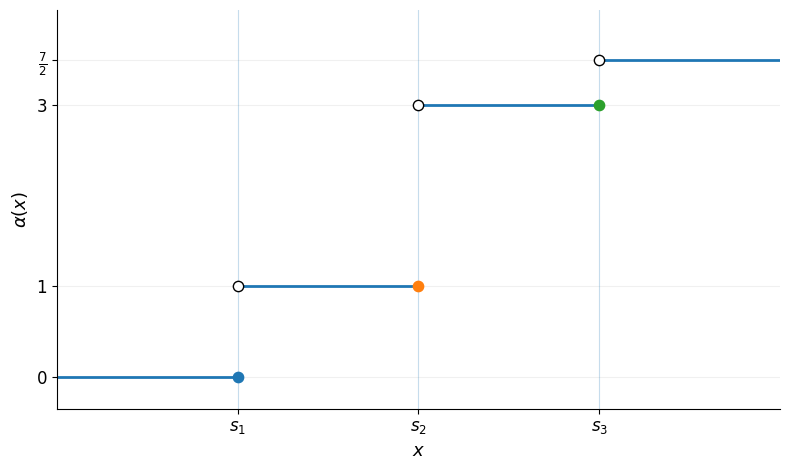
\includegraphics[width=0.5\textwidth]{
        CH6/images/Graph of a(x).png
    }
    \end{center}
\end{example}

\begin{theorem} \leavevmode \\
    \label{Thm6.15}
    Suppose $f: [a,b] \to \R$ is bounded, $s \in (a,b),$ $f$ is right continuous at $s$, and $\alpha(x) = I(x-s)$. Then $f \in R_\alpha[a,b]$ and $\int_a^b fd\alpha = f(s).$
\end{theorem}

\begin{proof}
    In what follows, we will introduce a sequence of partitions $(P_n)$ in $\Pi [a,b]$ such that 
    $$\lim_{n\to \infty} \left[U(f, \alpha, P_n) - L(f, \alpha, P_n)\right] = 0 \text{ and } \lim_{n\to \infty}U(f, \alpha, P_n) = \lim_{n\to\infty} L(f, \alpha,P_n) = f(s).$$
    This, according to the sequential criterion of integrability, tells us that 
    $$f \in R_\alpha [a,b] \text{ and } \int_a^b fd\alpha = f(s).$$
    Let $N$ be large enough so that $s + \frac{1}{N} < b.$ For each $n \geq N,$ let 
    $$P_n = \set{a, s, s+\frac{1}{n}, b}.$$
    We have 
    $$U(f, \alpha, P_n) = \sum_{k=1}^{3}M_k \Delta \alpha_k = M_2 \Delta \alpha_2 = \left[\sup_{s \leq x \leq s+ \frac{1}{n}}f(x)\right](1) = \sup_{s \leq x \leq s + \frac{1}{n}}f(x)$$
    $$L(f, \alpha, P_n) = \sum_{k=1}^{3}m_k \Delta \alpha_k = m_2 \Delta \alpha_2 = \left[\inf_{s \leq x \leq s+\frac{1}{n}}f(x)\right](1) = \inf_{s\leq x \leq s+ \frac{1}{n}}f(x).$$
    Therefore,
    $$\lim_{n\to \infty}U(f, \alpha, P_n) = \lim_{n\to \infty} \sup_{s \leq x \leq s + \frac{1}{n}}f(x) = f(x)$$
    $$\lim_{n \to \infty} L(f, \alpha, P_n) = \lim_{n \to \infty}\inf_{s \leq x \leq s+\frac{1}{n}}f(x) = f(x).$$
    Here, we are using the fact that $f$ is continuous at $s$, but right continuity would have been enough. We conclude that $\lim_{n \to \infty}\left[U(f, \alpha, P_n)- L(f, \alpha, P_n)\right] = f(s) - f(s) = 0,$ so $f \in R_\alpha[a,b]$ and $\int_a^bf d\alpha = \lim U(f, \alpha, P_n) = f(s).$
    \qed
\end{proof}

\begin{theorem} \leavevmode \\
    \label{Thm6.16}
    Suppose $\forall n \geq 1, c_n \geq 0,$ $\sum_{n=1}^{\infty}c_n$ converges. Let $s_1 < s_2< ... $ be points in $(a,b), \alpha:[a,b] \to \R, \alpha(x) = \sum_{n=1}^{\infty} c_n I(x-s_n),$ and $f:[a,b] \to \R$ be continuous. Then
    $$f\in R_\alpha[a,b] \text{ and } \int_a^bf d \alpha = \sum_{n=1}^{\infty}c_nf(s_n).$$
\end{theorem}